\documentclass[12pft, english]{article}
% \usepackage{apacite}
\RequirePackage[]{filecontents}
\usepackage[numbers]{natbib}
\usepackage{graphicx}
\graphicspath{ {./} }
\usepackage{url}
\usepackage[]{multicol}
\usepackage[strings]{underscore}
\usepackage[a4paper, bindingoffset=0.0in, left=0.5in, right=0.5in, top=1in, bottom=1in]{geometry}
\usepackage{xcolor}
\usepackage[]{amsfonts}
\usepackage[]{amsmath}
\usepackage[nottoc,numbib]{tocbibind}
\definecolor{pageGrey}{HTML}{111111}
%\pagecolor{pageGrey}
%\color{white}
\linespread{1.5}
\setlength{\columnseprule}{0.4pt}
\title{%
  Determining the input variables of a Multiplicative Congruential Generator \\
  \large Mathematics Internal Assessment}

\author{knv718}
\date{March 19th 2024}



\begin{filecontents}{\jobname.bib}
@book{example,
    author ="Michel Goossens and Frank Mittlebach and Alexander Samarin",
    title = "The Latex Companion A",
    year = "1993",
    publisher = "Addison-Wesley",
    address = "Reading,  Massachusetts"
}

@misc{waterlooMCG,
    author = "University Of Waterloo Math Department",
    title = "generating Random Numbers",
    howpublished = {\url{https://wiki.math.uwaterloo.ca/statwiki/index.php?title=generating_Random_Numbers#Inverse_Transform_Method}},
    year = "2009",
    publisher = "University Of Waterloo",
    address = "Waterloo, Canada"
}

@misc{jukSource,
    author =  "Juk Developers",
    title =  "playlist.cpp",
    howpublished = {\url{https://github.com/KDE/juk/blob/master/playlist.cpp#L676}},
    year = "2024",
    publisher = "KDE Foundatation",
    address = "Berlin Germany",
}

@article{fallOntoPlanes,
    author = "George Marsaglia",
    title =  "Random Numbers Fall Mainly In The Planes",
    journal = "Mathematics research Laboratory, Boeing Scientific Research Laboratories ",
    year = 1968
}

@article{linuxRNG,
    author = "Huzaifa Sidhurwala",
    title = "Understanding Random Number Generators and their Limitations, In Linux",
    journal = "Red Hat Blog",
    year = 2019
}
@misc{modArth,
    author = "Art Of Problem Solving",
    title = "Modular Arithmetic/Introduction",
    howpublished = {\url{https://artofproblemsolving.com/wiki/index.php/Modular_arithmetic/Introduction}},
    year = 2024,
}

@misc{utahMod,
    author = "Utah State University",
    title = "Modular Arithmetic Properties",
    howpublished = {\url{http://5010.mathed.usu.edu/Fall2019/SSwallow/ModProperties.html}},
    year = 2024
}

@misc{cornelMod,
    author = "Cornell University",
    title = "Everything You Need To Know About Modular Arithmetic",
    howpublished = {\url{https://pi.math.cornell.edu/~morris/135/mod.pdf}},
    year = 2006
}

@misc{standChinese,
  author = "Standford University",
  title = "The Chinese Remainder Theorem",
  howpublished = {\url{https://crypto.stanford.edu/pbc/notes/numbertheory/crt.html}},
  year = 2024
}

@misc{steinAlgo,
  author = "Algorithmica.org",
  title = "Bineary GDC",
  howpublished = {\url{https://en.algorithmica.org/hpc/algorithms/gcd/}},
  year = 2024
}

@article{reteamHal,
  author = "Haldir[RET]",
  title = "How to Crack A Linear Congruential Generator",
  journal = "reteam.org",
  year = 2004,
  howpublished = {\url{https://www.reteam.org/papers/e59.pdf}},
  note = " https://www.reteam.org/papers/e59.pdf"
}

@misc{wikiSpec,
  author = "Wikipedia Foundation",
  title = "Spectal Test",
  howpublished = {\url{https://en.wikipedia.org/wiki/Spectral_test}},
  year = 2024
}

@misc{waterlooLCG}


\end{filecontents}

% An article needs, author, title, journal, year,


\begin{document}
\maketitle

\pagebreak

\tableofcontents
\pagebreak

\begin{multicols}{2}
  \section{Introduction}
  Ever since I was a young child the concept of random has amazed me. Randomness could at times not seem random, for example, number generators, which are often pseudo-random number generators which are not particularly random. These pseudo-random number generators are not truly random, but rather just a mathematical equation which is being done iteratively, and if the developer was forward-thinking, it used a different seed (seed is the first value) every time too. \\
  Now among random number generators, there is a particularly common one called the Multiplicative Congruential Generator (MCG for short), it has been extensively used for various tasks that could require a lot of random numbers, that only need to be ``random enough''. For example, creating test data, or for things such as dice rolling in games. There is also another type of random number generator similar to it called the Linear Congruential Generator which is very similar in terms of how it functions.
  \section{Background}
  \subsection{Random Number Generators}
  \subsubsection{Multiplicitve Random Number Generator}
  Usually, an MCG works based on the equation \(x_{i+1} = (a \cdot x_{i}) \bmod m\). Where the next value is equal to the current value multiplied by a constant, the modulus is a constant too. \citep{waterlooMCG} \citep{fallOntoPlanes}
  \subsubsection{Linear Congruential Generators}
  In contrast, an LCG (Linear Congruential Generator) works in a very similar way, just adding a constant before the modulus operation. Its equation looks like \(x_{i+1} = (a \cdot x_{i} +b ) \bmod m\) \citep{waterlooMCG}
  \subsubsection{How LCG/MCG's are used}
  Linear/Multiplicative congruential generators are used in a variety of settings, from Monte Carlo simulations \citep{fallOntoPlanes}, to the shuffle function in music players \citep{jukSource}, these are just the implementations that are public and known about. Considering that these types of random number generators are also used in glibc's \citep{linuxRNG} random function, no one knows just how many things use these types of generators for their random numbers. So the implication of these random number generators not being random would have an unknown impact on the world.
  \subsubsection{Flaws of LCG/MCG's}
  Now these types of linear congruential generators have some flaws that were found by Gorge Marsaglia \citep{fallOntoPlanes}. That is, if you know how to arrange these numbers on a 3d object, all of the said numbers will fall upon \(\sqrt[n]{{n}! \cdot m}\) hyperplanes \citep{fallOntoPlanes}. A hyperplane is a plane of \(n-1 \) dimensions, with \(n\) being the number of dimensions. They essentially just cut the space into two ``parts''. As George Marsaglia put it, ``the points are about as randomly spaced in the unit n-cube as the atoms in a perfect crystal at absolute zero''. Later on in his paper, he goes over a method that can be used to determine the inputs to such an equation. \\
  In the quote, they mean they are perfectly spaced, and follow a pattern. Below is an a spectral test, which is used to see how ``random'' a random number generator is. The more ``random'' the spacing, the better the random number generator is. The image is from Wikipedia. \citep{wikiSpec}.
  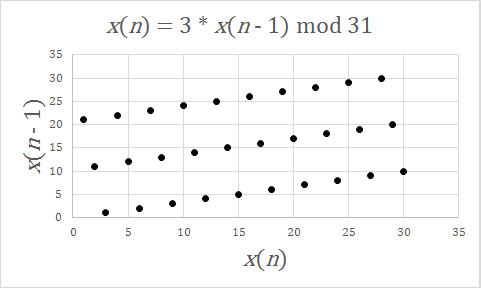
\includegraphics[width=4in]{Spectral_Test}
  \subsection{Modular Arithmetic}
  Modular arithmetic, as well as its properties, play an important role in both the generation and solving of linear/multiplicative congruential generators. The equations themselves use modular arithmetic, so knowing how it works, as well as its properties will prove useful when solving for the variables. \citep{modArth}
  \subsubsection{Residues}
  An important concept in modular arithmetic is residues, a residue is what is left when you subtract the modulo value as much as you can, before subtracting anymore would result in a negative number. It is also called the remainder in the context of division. \\
  An example of a residue would be, \( 10 \bmod 3\), which would have a residue of 1, as \(10 - ( 3 + 3 + 3 ) = 1\), subtracting anymore would result in a negative number. Thus the residue is 1. It is also important to note that a residue can be 0, such is the case of \( 12 \bmod 3\), where \( 12 - ( 3 + 3 + 3 + 3 ) = 0\), this is a case where the residue is equal to 0. \citep{modArth}
  \subsubsection{Congruence}
  We say numbers, or equations are congruent to one another when all of the residues/remainders of that value modulo a constant are the same. It is often shown through the sign \( \equiv \). An example of it being used correctly would be the equation; \( 2 \equiv 7 \equiv 12 (\bmod 5)\), as each of the values \( \bmod 5\) will have the same result, meaning they are congruent. \citep{modArth}
  \subsubsection{Relations}
  The relation between \(x \equiv b (\bmod m)\) and \(x = b (\bmod m )\). The first one is for equivalence. In comparison the second equation is equality. As a note from Cornell University put it; \\ ``\(x = b (\bmod m)\) is the smallest positive solution to the equation \( x \equiv b (\bmod m)\)'' \cite{cornelMod}
  \subsubsection{Rules to note:}
  Sum Rule: if \(a \equiv b ( \bmod m)\), and \(c \equiv d (\bmod m)\) then \( a + c \equiv b + c(\bmod m)\) \cite{cornelMod} \\ \\
  Multiplication Rule: if \(a \equiv b (\bmod m)\) and if \(c \equiv d (\bmod m)\) then \( a \cdot c \equiv b \cdot d (\bmod m)\)  \cite{cornelMod} \
  \subsubsection{Otherways it can be written }
  Another way in which \( a \equiv b (\bmod m)\) can be written is \(a = k \cdot m + b\), where \(k\) is an arbitrary integer. Yet another way it can be written is \(n | (a-b) \), which means, \(a-b\) is a multiple of \(n\). These becomes very useful when solving for the variables later on.

  \subsubsection{Chinese Remainder Theorm}
  Chinese remainder theorem is a surprise tool that will help us later on. Chinese remainder therom is a method to solve for \(x\) in a system of equations which are written as such; \(x = q_{n} (\bmod m_{n})\). Ben Lynn of Standford University states it;
  \[x = q_{1} (\bmod m_{1})\]
  \[x = q_{n} (\bmod m_{n})\]
  \citep{standChinese}
  For our purposes, only \(q_{n}\) changes, as the value of \(m\) stays constant. This means our equations will resemble;
  \[x = q_{1} (\bmod m)\]
  \[x = q_{n} (\bmod m)\]
  But because \(q_{n}\) is simply a constant multiplied by the previous number, like;
  \[q_{n} = a \cdot g \]
  Where \(g\) is the last value, and \(a\) is a constant whole number integer. \\
  So this means our equation looks like;
  \[ q_{i} = a \cdot g (\bmod m)\]
  From this, it has been said that we can use some special trickery (sum rule) to figure out the value of \(a\). However, brute forcing is a valid method, and in many cases is much simpler.
  \subsubsection{Brute Forcing}
  Brute force is a method of trial and error, where different values are continously tried until a value works.

  \subsection{Miscellaneous}
  \subsubsection{Determinate of a Matrix}
  An important tool that we will need in order to find the inital values of the the random generators is called the ``Determinate'', often times the determinate of the matrix is described as the volume/area of the matrix. But this definition does not do it justice, nor does it help in terms of understanding it. \\
  To explain it, we will discuss it in the context of a 2x2 matrix, on a 2d plane, in 2d space. From there we can abstract our understandings to 3d space. \\
  To start, let's talk about the unit square, a square which is one unit long, and one unit wide. It has an area of one. \\
  Now we also have a 2x2 matrix, let's call it \(A\), this matrix shall represent our hopes, dreams, and the transformations (Scaling, rotating, translations, etc) applied to the ``world'' that the unit square lives in. Now let's say we apply these transformations to the unit square, it's area will probbaly change, as its shape changes. Let's say it changes to 3, that means its area was changed by a factor of three. Now any thing in this world, which experienced this transformation would also be scaled by a factor of three. \\
  But where did the 3 come from? Well the 3 is the determinate of the matrix, and the factor by which which everything changes.  \\
  So this means that the determinate of the matrix \(A\) is like the factor by which the area changes. Some people also say the determinate of the matrix is the the area of the matrix. \\
  Now by abstracting it to 3d space, we change area to volume, use a 3x3 matrix instead, and the rest of the principles stay the same.

  \subsection{Method of Solving }
  % originally \citep{reteamHal}
  The original paper by George Marsaglia \citep{fallOntoPlanes} mentioned a method which could be used to solve for the original inputs given a sufficient amount of input. This was then expanded upon by Haldir \citep{reteamHal}. The expanded-upon method showcased by Haldir will be used, although first how it works will be explained in this section.
  \subsubsection{Forming the Matrix}
  To begin solving for the input values you need to obtain 6 values from the generator, let these values be \( \{ 1 \leq i \leq 6 \} , \{1 \leq x_{i} | x_{i} \in \mathbb{Z}^{+}\} \). Let \( i \) be the index of the value, and \( x_{i}\) be the value. \\
  The method that was used in this investigation, and the method used in Marsaglia's, and Haldir's papers differ here. In their papers they set up the matrix as; \citep{fallOntoPlanes} \citep{reteamHal}
    \[
    \begin{bmatrix}
      x_{1} & x_{2} & 1 \\
      x_{2} & x_{3} & 1 \\
      x_{3} & x_{4} & 1 \\
    \end{bmatrix}
  \]
    However, during my inital calculations I had discovered that a different arragmenet of values also worked;
  \[
    \begin{bmatrix}
      x_{1} & x_{2} & 1 \\
      x_{3} & x_{4} & 1 \\
      x_{5} & x_{6} & 1 \\
    \end{bmatrix}
  \]

  Following this discovery, I used this arrangment of values for the rest of the calculations.

  \subsubsection{Finding \(m\)}
  Now that the matrix has been arranged as;
 \[
    \begin{bmatrix}
      x_{1} & x_{2} & 1 \\
      x_{3} & x_{4} & 1 \\
      x_{5} & x_{6} & 1 \\
    \end{bmatrix}
  \]
  We need to find the determinate, as Haldir, and Marsaglia found, the determinate of this matrix is an integer multiple of the value of \(m\) in the equation of the LCG/MCGs. \\
  Before finding the determinate, for the sake of simplicity, we will assign variable names to each of the points in the matrix before replacing them with the actual numbers. They will be labelled as such;
  \[
    A =
    \begin{bmatrix}
      a_{1} & a_{2} & a_{3} \\
      b_{1} & b_{2} & b_{3} \\
      c_{1} & c_{2} & c_{3} \\
    \end{bmatrix}
  \]

  \[
    \det(A) =
    a_{1} \cdot
    \begin{vmatrix}
      b_{2} & b_{3} \\
      c_{2} & c_{3} \\
    \end{vmatrix}
    -
    a_{2}
    \cdot
    \begin{vmatrix}
      b_{1} & b_{3} \\
      c_{1} & c_{3} \\
    \end{vmatrix}
    +
    a_{3}
    \begin{vmatrix}
      b_{1} & b_{2} \\
      c_{1} & c_{2} \\
    \end{vmatrix}
  \]
  \[
    \det(A) = a_{1} \cdot (b_{2} \cdot c_{3} - b_{3} \cdot c_{2}) - a_{2}(b_{1} \cdot c_{3} - b_{3} \cdot c_{1}) + a_{3}(b_{1} \cdot c_{2} - b_{2} \cdot c_{1})
  \]
  Then after replacing the letters a,b, and c, you end up with the equation below.
  \[
  = x_{1} \cdot ((x_{3} \cdot 1)- (x_{5} \cdot 1)) - x_{2} \cdot ((x_{2} \cdot 1) - (x_{4} \cdot 1)) +((x_{2} \cdot x_{5}) - (x_{3} \cdot x_{4}))
  \]
  After simplifying this equation one will end up with;
  \[
  \det(A) = x_{1} \cdot (x_{3}- x_{5}) - x_{2} \cdot (x_{2} - x_{4}) + ((x_{2} \cdot x_{5}) - (x_{3} \cdot x_{4}))
  \]
  Now that we have the determinate for one set of numbers, we need to repeat it a lot of times and record all of the determinates. The theoretical minimum number of determinates needed is found in George Marsaglia's paper \citep{fallOntoPlanes}. It has a table of the number needed, for this investigation, the process will just be repeated 12.

  Now that we have obtained some determinates, we will need to find their largest common factor. I suggest using a compute program to find the factors of each number, and then save them. After all of the factors have been found, find the largest common number between them all. An example will be shown below with arbitrary numbers 500, 525, 450, 700
  \begin{flalign}
    & 500 : 1, 2, 4, 5, 10, 20, 25, 50, 100, 125, 250, 500 \\
    & 525 : 1, 3, 5, 7, 15, 21, 25, 35, 75,  105, 175, 525 \\
    & 450 : 1, 2, 3, 5, 6, 9, 10, 15, 18, 25, 30, 45, 50,..., 450 \\
    & 700 : 1, 2, 4, 5, 7, 10, 14, 20, 25, 28, 35, 50, ..., 700
  \end{flalign}
  In the case of the numbers above, the greatest common factor is 25. Thus the value of \(m\) in the equation of an MCG/LCG is 25.

  \subsubsection{Solving for \(a\) in an MCG}
   To solve for the remaining variables of an LCG, we will use the equation
  \[ x_{i} = (x_{i-1} \cdot a ) \bmod m\]
  Since we have \(m\), and have \(x_{i}\), we just have to solve for \(a\), which is trivial, it can be done using the Chinese Remainder Theorem, or brute force.  The value of \(a\) can simply be brute forced.
  \section{Investigation}
  To begin, a multiplicative congruential generator will be used to generate 72 numbers. Then those numbers will be used to find the original inputs to the generator, to check if the inputs are correct, the values which were found will be used as inputs to the multiplicative congruential generator.
  \subsection{Values}
  The 72 numbers which were found are stated below; \\
  547, 91, 73, 200, 19, 159, 109, 157, 170, 90, 209, 61, 144, 39, 182, 146, 189, 38, 107, 7, 103, 129, 180, 207, 122, 77, 78, 153, 81, 167, 76, 3, 14, 206, 47, 149, 203, 33, 154, 156, 95, 162, 123, 152, 6, 28, 201, 94, 87, 195, 66, 97, 101, 190, 113, 35, 93, 12, 56, 191, 188, 174, 179, 132, 194, 202, 169, 15, 70, 186, 24, 112 \\
  These values will be used for the calculation of the input values of the MCG.
  \subsection{Setting up the Matrixes}
  Now we will need to setup the 12 matrixes we will be using to find the value of \(m\). The matrixes will be setup as such
  \[
    A =
    \begin{bmatrix}
      547 & 91  & 1 \\
      73  & 200 & 1 \\
      19  & 159 & 1\\
    \end{bmatrix}
  \]

  \[
    B =
    \begin{bmatrix}
      109 & 157 & 1 \\
      170 & 90  & 1 \\
      209 & 61  & 1\\
    \end{bmatrix}
  \]


  \[
    C =
    \begin{bmatrix}
      144 & 39  & 1 \\
      182 & 146 & 1 \\
      189 & 38  & 1\\
    \end{bmatrix}
  \]

  \[
    D =
    \begin{bmatrix}
      107 & 7   & 1 \\
      103 & 129 & 1 \\
      180 & 207 & 1\\
    \end{bmatrix}
  \]

  \[
    E =
    \begin{bmatrix}
      122 & 77  & 1 \\
      782 & 153 & 1 \\
      81  & 167 & 1\\
    \end{bmatrix}
  \]

  \[
    F =
    \begin{bmatrix}
      76  & 3   & 1 \\
      14  & 206 & 1 \\
      47  & 149 & 1\\
    \end{bmatrix}
  \]

  \[
    G =
    \begin{bmatrix}
      203 & 33  & 1 \\
      154 & 156 & 1 \\
      95  & 162 & 1\\
    \end{bmatrix}
  \]

  \[
    H =
    \begin{bmatrix}
      123 & 152 & 1 \\
      6   & 28  & 1 \\
      201 & 94  & 1\\
    \end{bmatrix}
  \]

  \[
    I =
    \begin{bmatrix}
      87  & 195 & 1 \\
      66  & 97  & 1 \\
      101 & 190 & 1\\
    \end{bmatrix}
  \]

  \[
    J =
    \begin{bmatrix}
      113 & 35  & 1 \\
      93  & 12  & 1 \\
      56  & 191 & 1\\
    \end{bmatrix}
  \]

  \[
    K =
    \begin{bmatrix}
      118 & 174 & 1 \\
      179 & 132 & 1 \\
      194 & 202 & 1\\
    \end{bmatrix}
  \]

  \[
    L =
    \begin{bmatrix}
      169 & 15  & 1 \\
      70  & 186 & 1 \\
      24  & 112 & 1\\
    \end{bmatrix}
  \]

  \subsection{Getting the Determinates of the Matrixes}
  Now that we've arranged all the matrixes we need to get the absolute value of their determinates, absolute values for simplicity sake later on when we need to find the factors. The function \(\det(A)\) shall represent it, letting \(A\) be the matrix.
  \[
    \det(A) =
    547 \cdot
    \begin{vmatrix}
      200 & 1 \\
      159 & 1 \\
    \end{vmatrix}
    -
    91 \cdot
    \begin{vmatrix}
      73 & 1 \\
      19 & 1 \\
    \end{vmatrix}
    +
    \begin{vmatrix}
      547 & 91 \\
      19 & 159 \\
    \end{vmatrix}
  \]
  \[
    \det(A) = 25320
  \]

  \[
    \det(B) =
    109 \cdot
    \begin{vmatrix}
      90 & 1 \\
      61 & 1 \\
    \end{vmatrix}
    -
    157 \cdot
    \begin{vmatrix}
      170 & 1 \\
      209 & 1 \\
    \end{vmatrix}
    +
    \begin{vmatrix}
      109 & 157 \\
      209 & 61 \\
    \end{vmatrix}
  \]
  \[
    \det(B) = 844
  \]

  \[
    \det(C) =
    144 \cdot
    \begin{vmatrix}
      146 & 1 \\
      38 & 1 \\
    \end{vmatrix}
    -
    39 \cdot
    \begin{vmatrix}
      182 & 1 \\
      189 & 1 \\
    \end{vmatrix}
    +
    \begin{vmatrix}
      144 & 39 \\
      189 & 38 \\
    \end{vmatrix}
  \]
  \[
    \det(C) = 4853
  \]

  \[
    \det(D) =
    107 \cdot
    \begin{vmatrix}
      129 & 1 \\
      207 & 1 \\
    \end{vmatrix}
    -
    7 \cdot
    \begin{vmatrix}
      103 & 1 \\
      180 & 1 \\
    \end{vmatrix}
    +
    \begin{vmatrix}
      107 & 7 \\
      180 & 207 \\
    \end{vmatrix}
  \]
  \[
    \det(D) = 9706
  \]

  \[
    \det(E) =
    122 \cdot
    \begin{vmatrix}
      153 & 1 \\
      167 & 1 \\
    \end{vmatrix}
    -
    77 \cdot
    \begin{vmatrix}
      78 & 1 \\
      81 & 1 \\
    \end{vmatrix}
    +
    \begin{vmatrix}
      122 & 77 \\
      81 & 167 \\
    \end{vmatrix}
  \]
  \[
    \det(E) = 844
  \]

  \[
    \det(F) =
    76 \cdot
    \begin{vmatrix}
      206 & 1 \\
      149 & 1 \\
    \end{vmatrix}
    -
    3 \cdot
    \begin{vmatrix}
      14 & 1 \\
      47 & 1 \\
    \end{vmatrix}
    +
    \begin{vmatrix}
      76 & 3 \\
      47 & 149 \\
    \end{vmatrix}
  \]
  \[
    \det(F) = -3165
  \]

  \[
    \det(G) =
    203 \cdot
    \begin{vmatrix}
      156 & 1 \\
      162 & 1 \\
    \end{vmatrix}
    -
    33 \cdot
    \begin{vmatrix}
      154 & 1 \\
      95 & 1 \\
    \end{vmatrix}
    +
    \begin{vmatrix}
      203 & 33 \\
      95 & 162 \\
    \end{vmatrix}
  \]
  \[
    \det(G) = 6963
  \]

  \[
    \det(H) =
    123 \cdot
    \begin{vmatrix}
      28 & 1 \\
      94 & 1 \\
    \end{vmatrix}
    -
    152 \cdot
    \begin{vmatrix}
      6 & 1 \\
      201 & 1 \\
    \end{vmatrix}
    +
    \begin{vmatrix}
      123 & 152 \\
      201 & 94 \\
    \end{vmatrix}
  \]
  \[
    \det(H) = 16458
  \]

  \[
    \det(I) =
    87 \cdot
    \begin{vmatrix}
      97 & 1 \\
      190 & 1 \\
    \end{vmatrix}
    -
    195 \cdot
    \begin{vmatrix}
      66 & 1 \\
      101 & 1 \\
    \end{vmatrix}
    +
    \begin{vmatrix}
      87 & 195 \\
      101 & 190 \\
    \end{vmatrix}
  \]
  \[
    \det(I) = 1477
  \]

  \[
    \det(J) =
    113 \cdot
    \begin{vmatrix}
      12 & 1 \\
      191 & 1 \\
    \end{vmatrix}
    -
    35 \cdot
    \begin{vmatrix}
      93 & 1 \\
      56 & 1 \\
    \end{vmatrix}
    +
    \begin{vmatrix}
      113 & 35 \\
      56 & 191 \\
    \end{vmatrix}
  \]
  \[
    \det(J) = 4431
  \]

  \[
    \det(K) =
    188 \cdot
    \begin{vmatrix}
      132 & 1 \\
      202 & 1 \\
    \end{vmatrix}
    -
    174 \cdot
    \begin{vmatrix}
      179 & 1 \\
      194 & 1 \\
    \end{vmatrix}
    +
    \begin{vmatrix}
      188 & 174 \\
      194 & 202 \\
    \end{vmatrix}
  \]
  \[
    \det(K) = 0
  \]

  \[
    \det(L) =
    169 \cdot
    \begin{vmatrix}
      186 & 1 \\
      112 & 1 \\
    \end{vmatrix}
    -
    15 \cdot
    \begin{vmatrix}
      70 & 1 \\
      24 & 1 \\
    \end{vmatrix}
    +
    \begin{vmatrix}
      169 & 15 \\
      24 & 112 \\
    \end{vmatrix}
  \]
  \[
    \det(L) = 15192
  \]

  Excluding the determinate(s) which are 0, we have the determinates, 25320, 844, 4853, 9706, 844, 3165, 6963, 16458, 1477, 4431, 15192.

  \subsection{Solving for the Inital Values}

  From the determinates of the matrix we can solve for \(m\), using the method which was previously stated. That is, to find the greatest common factor between all of the determinates. After solving for the greatest common factor, a value of \(211\) is obtained. That means that the equation of the MCG that is generating these values should look similar to \(x_{i+1} \equiv (a \cdot x_{i}) (\bmod {211})\). \\
  Using some of the equations previously mentioned, we can re-arrange them to craft the equation. \cite{reteamHal}
  \[ a \cdot x_{i - 1} \equiv x_{i} ( \bmod m )\]
  Since we know the value of \(m\) is 211, we can insert it into the equation, getting
  \[a \cdot x_{i-1} \equiv x_{i} (\bmod 211)\]
  To determine \(a\) we shall use 6 different values of \(x\), if the solved values of \(a\) are all the same, we will have found \(a\). The values used will be; 109, 157, 73, 200, 19, and 159. Putting these into equations we get the equations;
  \AtBeginEnvironment{align}{\setcounter{equation}{0}}
  \begin{gather*}
      157 \equiv 109 \cdot a (\bmod 211) \\
      200 \equiv 73 \cdot a (\bmod 211)  \\
      157 \equiv 109 \cdot a (\bmod 211) \\
    \end{gather*}

    By brute forcing these equations for the value of \(a\), a value of \(75\) is obtained.

    Thus the values of \(a\) is \(75\), and \(m\) is \(211\). You only need one value from the generator to predict all the values which come after it, so we have everything that is needed.

    \subsection{Checking the values}
    To check our values, we will need one value from the MCG to act as the seed, and then we'll need to solve for the next values, if the values line up, we'll know we have the correct values. Using the equation \(x_{i} = x_{i-1} \cdot a (\bmod m)\) we can solve for them. The value of \(x_{1}\) will be 547, as that is the first value to come out of the generator, the values of \(m\), and \(a\), have already been solved for, and were shown to be 211, and 75 respectively. This means we get an equation of \( x_{i} \equiv x_{i-1} \cdot 75 (\bmod 211)\). Inserting in 547, the number we get out is 91. Repeating that 10 times, we get the sequence; 547, 91, 73, 200, 19, 159, 109, 157, 170, 90. Which perfectly matches the order, and values that were extracted from the actual generator, meaning our values are correct.
    \subsection{Applications/Implications of knowing the inputs}
    There are many implications of being able to predict the next ``random'' number there are so many implications that we do not know just how far-reaching the consequences are. One of the implications as stated before is about about cryptography, as quite a few badly built cryptographic programs use Linear, and Multiplicative Congruential Generators as randomness generators. Another consequence is the use of random in video games, and computer graphics. In video games, they are often used to place objects or to randomize the behaviours of characters. Whilst in computer graphics random generators are used to seed the rendering equations to make renders seem more realistic, as there is ``random''. So these random number generators being predictable means that, these applications are not getting truly random values.


    \subsection{Limitations}
    However, there are many limitations of this method to determine the input variables using the outputs. The first and largest limitation is, determining whether an LCG/MCG is being used, as you would need access to the code of the application to determine whether an LCG/MCG is being used. The alternative method of spectral analysis to determine whether an LCG/MCG would require a significant number of data points, which may be unrealistic to collect. \\
    The next limitation would be the number of values needed, as extracting the required number of values needed would take a significant amount of time\\
    Then there is the time it would take to find the GCD of larger numbers, as computing the factors of numbers takes a sufficiently long time, and as the numbers grow larger, the time taken also grows. So if a lot of values were extracted, and thus determinates found, it would take quite a while to find the value of \(m\). However, the use of the Chinese Remainder Theorem and Stein's algorithm could potentially decrease the time taken. These algorithims would allow you to find the factors, and the value of \(m\) with far less brute forcing than otherwise. But it would still be incredibly difficult. \\


    \subsection{Extensions}
    There are many methods to extend this investigation, such as; investigating the use of Steins's algorithm, and Chinese Remainder Therom. Steins's algorithm is often used to find the greatest common denominator between two non-negative numbers \(u\), and \(v\) by repeatedly applying these identities;
    \begin{enumerate}
      \item Let \(gcd(a,b)\) be a function which returns the greatest integer by which both values can be divided which results in a positive integer
      \item \(gcd(0,b) = b\), and symmetrically; \(gcd(a,0) = a\)
      \item \(gcd(2a,2b) = 2 \cdot gcd(a,b)\)
      \item \(gcd(2a, b) = gcd(a,b)\) if \(b\) is odd,\\
            then \(gcd(a,b) = gcd(a,2b) \) if \(a\) is odd
      \item \(gcd(a,b) = gcd(|a-b|, min(a,b))\),\\
            if \(a\) and \(b\) are both odd
    \end{enumerate}
    (Note: Symmetrically in this context, means the other way around, as in the values swapped)
    Stein's algorithm is simply the continuous application of these rules until the \(gcd\) is found. \citep{steinAlgo}. The use of Stein's algorithm would be a great step forward when it comes to decreasing the time taken to find the value of \(m\). \\
    Continuing, Chinese Remainder Therom as previously mentioned could be used in order to make the calculations done by hand much faster. It could also be applied to solve for a Linear Congruential Generator. However, the existence of fast computers makes brute forcing a much more reasonable operation. Until the values are sufficiently large, where solving by hand is quicker. \citep{fallOntoPlanes} \\
    However, one extension which was taken in this paper, and should be further investigated is different arrangments of the values in the matrix. During this investigation, the liberty was taken to use a different arrangement of values in the matrix. It was found that the different arrangements worked, this shows that other variations of this setup could work.


\end{multicols}

%Some asdclaisdm \citep{example}
%\citet{waterlooMCG}
%\citet{whack}

\pagebreak


\bibliographystyle{plainnat}
\bibliography{\jobname}


\end{document}
